\subsection*{Общая характеристика работы}

\newcommand{\actuality}{{\textbf{Актуальность темы.}}}
\newcommand{\aim}{{\textbf{Целью}}}
\newcommand{\tasks}{{\textbf{задачи}}}
\newcommand{\defpositions}{{\textbf{Основные положения, выносимые на~защиту:}}}
\newcommand{\novelty}{{\textbf{Научная новизна:}}}
\newcommand{\influence}{{\textbf{Практическая значимость}}}
\newcommand{\reliability}{{\textbf{Достоверность}}}
\newcommand{\probation}{{\textbf{Апробация работы.}}}
\newcommand{\contribution}{{\textbf{Личный вклад.}}}
\newcommand{\publications}{{\textbf{Публикации.}}}
\floatname{algorithm}{Алгоритм}

\newtheorem{theorem}{Теорема}
%\newtheorem{algorithm}{Алгоритм}
\newtheorem{definition}[theorem]{Определение}
\newtheorem{assumption}[theorem]{Допущение}
\newtheorem{assumptionext}[theorem]{Допущение}
\newtheorem{lemma}[theorem]{Утверждение}

%Ляхов Андрей Игоревич

{\actuality}
В настоящий момент времени огромной популярностью обладают сервисы хранения и передачи видео по протоколу прикладного уровня HyperText Transfer Protocol (HTTP). Данное явление вызвано множеством факторов, такими как бурное развитие мобильных устройств, увеличение аудитории социальных сетей и их плотная интеграция с сервисами хранения видеоконтента, рост популярности дистанционного обучения, видеокурсов, видеолекций и т. д. Подобная комбинация факторов приводит к доминированию передачи видеоданных в современных телекоммуникационных системах.

Важной особенностью передачи видео по протоколу HTTP является наличие двух технологий организации передачи видеоданных: неадаптивная (HTTP Progressive Download) и адаптивная (HTTP Adaptive Streaming), представленные в стандарте Dynamic Adaptive Streaming over HTTP (DASH). В современных реалиях пользователи обладают высокой мобильностью, что приводит к использованию беспроводных сетей связи в качестве носителя информации. Рост объемов видеотрафика приводит к экстремальным нагрузкам на беспроводную сеть, что проявляется в появлении эффектов деградации качества обслуживания абонентов: увеличение длительности ожидания начала воспроизведения и прерывание проигрывания видеоконтента при просмотре.

Общая производительность беспроводных централизованных сетей во многом определяется аспектами работы с беспроводным каналом связи, а именно методом распределения частотно-временных ресурсов между пользователями. В современных стандартах связи распределение ресурсов осуществляет алгоритм планирования (планировщик), установленный на уровне доступа ко среде, базовой станции. Планировщики не регламентируются стандартами, и каждый производитель оборудования по собственному усмотрению выбирает принципы, в соответствии с которыми будет организовано распределение ресурсов радиоканала, что имеет непосредственное влияние на производительность системы в целом.

Таким образом, актуальной является задача анализа производительности и создания алгоритмов планирования для беспроводных централизованных сетей, которые обеспечивают высокую производительность и достаточный уровень качества восприятия при передаче видеоданных по протоколу HTTP.

%Большое количество усилий было направлено на изучение данной предметной области.
%В настоящей работе, для анализа производительности беспроводных сетей используется методы
При анализе производительности беспроводных централизованных сетей для передаче видео использовалась теория замкнутых систем массового обслуживания с конечным числом абонентов, проработанная A. Scherr, L. Kleinrock, В.М. Вишневским и А.И. Ляховым. Применение настоящей теории к анализу систем передачи видеоданных было представлено в ряде работ отечественных: Е.А. Бакин, Г.С. Евсеев, А.И. Парамонов, и зарубежных авторов: A. El Essaili, O. Oyman, V. Ramamurthi, исследующих производительность алгоритмов планирования для передачи видеоконтента. В большинстве подобных работ рассматривается неадаптивная технология передачи и предлагаются подходы для увеличения производительности в соответствии с рассматриваемым критерием качеством восприятия.

\aim\ настоящего диссертационного исследования является определение, вычисление и построение численных показателей максимально возможной производительности беспроводных централизованных телекоммуникационных систем при использовании адаптивной и неадаптивной технологии передачи видеоданных по протоколу HTTP, и предложение класса алгоритмов планирования распределения ресурсов беспроводного канала на базовой станции, производительность которых близка к максимально достижимой производительности беспроводных централизованных сетей.

Для~достижения поставленной цели необходимо решить следующие {\tasks}:
\begin{enumerate}
    \item Исследовать способы адаптивной и неадаптивной технологий передачи видеоданных по протоколу HTTP;
    \item Исследовать методы и критерии оценки качества восприятия видеоряда для адаптивной и неадаптивной передачи видеоданных и выделить факторы, обладающие наибольшим влиянием на качество восприятия;
    %\item Предложить критерии качества восприятия видеоданных для адаптивной и неадаптивной технологии передачи по протоколу HTTP;
    \item Ввести модель системы передачи видеоданных, включающую в себя модели компонентов системы передачи видео и беспроводной централизованной сети, и найти взаимосвязь между ее параметрами;
    \item Предложить аналитические оценки максимально возможной производительности введенной модели телекоммуникационной системы для исследованных критериев качества восприятия адаптивной и неадаптивной передачи видеоданных по протоколу HTTP;
    \item Разработать алгоритм планирования распределения ресурсов беспроводного канала связи на основе полученных аналитических результатов и продемонстрировать его производительность в сравнении с ними и существующими решениями.
\end{enumerate}

\textbf{Объект и предмет исследования}. Объектом исследования является беспроводная централизованная телекоммуникационная система с доминированием передачи видеоданных по протоколу HTTP.

Предмет исследования составляет алгоритм распределения частотно-временных ресурсов беспроводного канала связи на базовой станции при адаптивной потоковой передаче видеоданных по протоколу HTTP.

\textbf{Методы исследования.} При получении основных результатов работы использовались общие методы теории вероятностей и математической статистики, теории случайных процессов, методы математической оптимизации, в частности нелинейного и невыпуклого программирования, а также методы имитационного моделирования.

\novelty
\begin{enumerate}
    \item Построена трехкомпонентная модель системы передачи видеоданных по протоколу HTTP в беспроводных централизованных сетях связи, позволяющая провести аналитические исследования и сравнение производительности алгоритмов распределения ресурсов беспроводного канала;
    \item Найдена взаимосвязь между характеристиками системы передачи информации и проигрывания видеоряда при передаче видео по HTTP протоколу;
    \item Предложен способ вычисления нижней границы для нормированного отношения длительностей буферизации и просмотра при неадаптивной передачи видеоданных по всевозможным алгоритмам планирования, удовлетворяющим введенной модели;
    \item Предложен и реализован алгоритм планирования, минимизирующий нормированное отношение длительностей буферизации и просмотра при неадаптивной передачи видеоданных;
    \item Найдена нижняя граница для отношения длительностей буферизации и просмотра с учетом средней битовой скорости потока при адаптивной передаче видеоданных по всевозможным алгоритмам планирования и адаптации видеоряда, удовлетворяющим введенной модели.
\end{enumerate}

\influence\ диссертационной работы. Полученные в диссертационной работе результаты позволяют повысить производительность алгоритмов планирования распределения ресурсов беспроводного канала, и, как следствие, системы передачи информации в целом, для передачи видео по протоколу HTTP, что способствует увеличению емкости беспроводных систем. Так же полученные результаты могут быть использованы для формирования требований к разрабатываемым стандартам связи текущих и последующих поколений.

\reliability. Результаты, полученные в диссертационной работе, согласуются с известными исследованиями передачи видеоданных по протоколу HTTP в беспроводных сетях. Основные результаты опубликованы в рецензируемых журналах и доложены на крупных международных конференциях.

\probation\ Основные результаты работы докладывались и обсуждались на следующих конференциях и симпозиумах в период с 2013 по 2017 гг.: на научных сессиях ГУАП; на конференции <<СПИСОК-2014>> на $15$-й конференции <<Conference of Open Innovations Association FRUCT>>; на $16$-м симпозиуме <<Problems of Redundancy in Information and Control Systems>>.

\textbf{Внедрение результатов.} Результаты работы были использованы в рамках проекта <<Разработка технических решений по построению внутриобъектовой сети мобильной радиосвязи>> ПАО <<Информационные телекоммуникационные технологии>>. Кроме того, результаты работы используются в учебном процессе кафедры инфокоммуникационных систем и кафедры безопасности информационных систем ГУАП.

\contribution\ Все результаты, представленные в тексте диссертационной работы, получены автором лично.

\publications\ Материалы, отражающие основное содержание и результаты диссертационной работы, опубликованы в $14$ печатных работах. Из них $2$ работы опубликованы в рецензируемых научных журналах, утвержденных в перечне ВАК, и $4$ работ опубликованы в журналах, индексируемых в Scopus.

\defpositions
\begin{enumerate}
    \item Модель беспроводной централизованной системы связи при передаче видеоданных по протоколу HTTP, позволяющая производить аналитические исследования алгоритмов планирования распределения ресурсов беспроводного канала .
    \item Взаимосвязь характеристик беспроводной централизованной сети и воспроизведения видеоряда при передачи видео по протоколу HTTP.
    \item Нижняя граница для нормированного отношения длительностей буферизации и просмотра по всевозможным алгоритмам планирования, удовлетворяющим введенной модели, при передаче неадаптивных видеопотоков.
    \item Алгоритм планирования распределения ресурсов беспроводного канала для минимизации нормированного отношения длительностей ожидания и просмотра при передаче неадаптивных видеопотоков.
    \item Нижняя граница для отношения длительностей буферизации и просмотра с учетом средней битовой скорости потока при адаптивной передачи видеоданных по всевозможным алгоритмам планирования и адаптации видеоряда, удовлетворяющим введенной модели.
\end{enumerate}
 % Характеристика работы по структуре во введении и в автореферате не отличается (ГОСТ Р 7.0.11, пункты 5.3.1 и 9.2.1), потому её загружаем из одного и того же внешнего файла, предварительно задав форму выделения некоторым параметрам

%Диссертационная работа была выполнена при поддержке грантов ...

{\textbf{Объем и структура работы.}} Диссертация состоит из введения, четырёх разделов, заключения и двух приложений. Полный объём диссертации составляет 142 страницы с 28 рисунками и 7 таблицами. Список литературы содержит 66 наименований.

%\newpage
\subsection*{Содержание работы}
Во \textbf{\textit{введении}} обоснована актуальность исследования алгоритмов распределения ресурсов радиоканала при передаче видео по протоколу HTTP в беспроводных централизованных сетях связи, представлена научная новизна диссертационной работы и ее практическая ценность сформулированы основные положения, выносимые на защиту, а также приведено краткое содержание диссертационной работы по разделам.

%------------------------------------------------------------------------------------------------------------------------------------%

В \textbf{\textit{первом разделе}} рассматриваются особенности организации передачи видеоданных по протоколу HTTP в современных телекоммуникационных сетях, обозреваются существующие технологии передачи видеоданных и методологии оценки качества восприятия видеоданных при их прохождении через сеть передачи данных. На основе проведенного обзора в формируются модели системы передачи видеоданных и критерии качества восприятия видеопотоков.

%Рассматривается типовая модель системы передачи видео по HTTP, состоящая из видео контент сервера, сети передачи информации и пользовательских устройств. В данной модели управляющим компонентом является пользовательское устройство, так как именно оно производит формирование последовательности запросов на видеоданные к Видео Контент Серверу, и, как следствие, требований к сети передачи информации по обслуживанию соединения.

Производительность телекоммуникационных систем при передаче видеоданных определяется удовлетворенностью пользователей воспроизведением видео при прохождении через сеть. Удовлетворенность пользователя возможно охарактеризовать критериями качества восприятия (Quality of Experience), которые позволяют на основе некоторого массива объективных показателей работы сети оценить субъективное восприятие пользователем качества обслуживания. Общепринятым подходом к оценке качества восприятия является Mean Opinion Score (MOS)~--~семейство сложных функций, позволяющее оценить удовлетворенность пользователя по шкале от одного до пяти в зависимости от огромного массива статистик воспроизведения видеопотока и технологии передачи видео (адаптивной и неадаптивной). В результате обзора известных видов функций MOS и их аппроксимаций были выделены основные факторы, влияющие на качество восприятия видеоданных в зависимости от технологий передачи:
\begin{itemize}
	\item Фактор длительности ожидания (буферизации) в течении просмотра видеопотока: \textbf{Неадаптивная} и \textbf{Адаптивная} технологии;
	\item Средняя битовая скорость просмотренного видеопотока: \textbf{Адаптивная}.
\end{itemize}
Было установлено, что удовлетворенность пользователя просмотром, и, как следствие, производительность телекоммуникационной системы, обратно пропорциональна значению фактора буферизации и прямо пропорциональна средней битовой скорости потока. Известны два критерия качества восприятия, характеризующие фактор буферизации для конкретного пользователя $i$:
\begin{itemize}
	\item \textit{Нормированное отношение длительностей буферизации и просмотра}:
	\begin{equation}
    	\label{eq:g_def}
    	g_i = \lim\limits_{T\rightarrow\infty} \frac{b_i^T}{w_i^T + b_i^T},
    \end{equation}
    где $b_i^T$~--~общая длительность буферизации пользователя $i$ за время $T$, $w_i^T$~--~общая длительность просмотренного видео пользователем $i$ за время $T$,
	\item \textit{Отношение длительностей буферизации и просмотра}:
	\begin{equation}
    	\label{eq:q_def}
    	q_i = \lim\limits_{T\rightarrow\infty} \frac{b_i^T}{w_i^T}.
    \end{equation}
\end{itemize}

В настоящее время широко исследована производительность беспроводных систем при использовании неадаптивной технологии для критерия качества (\ref{eq:q_def}), однако, для критерия (\ref{eq:g_def}) отсутствуют исследования производительности беспроводных систем связи при передаче видеоданных по протоколу HTTP.

Далее в диссертационном исследовании проводится анализ производительности беспроводной системы связи для критерия качества (\ref{eq:g_def}) при использовании неадаптивной технологии передачи видеоданных, и критерия качества (\ref{eq:q_def}) при адаптивной технологии передачи видеоданных.

%В настоящее время технология передачи видеоданных по протоколу HTTP регламентируется стандартом Dynamic Adaptive Streaming over HTTP (DASH), предложенным в 2012-м году Международной Электротехнической Комиссией.

%Данный стандарт передачи информации построен на основе протоколов прикладного и транспортного уровней HTTP и Transmission Control Protocol (TCP) соотвественно. Важной отличительной особенностью использования данных протоколов является инвариантность к сети передачи информации: она может иметь произвольную структуру и построена на любом физическом принципе, и для успешной передачи данных необходимо лишь обеспечение корректной работы протокола HTTP. Как следствие, информация при прохождении через подобную сеть не может быть потеряна, ввиду работы TCP прокола.

%Стандарт DASH регламентирует особый формат хранения и представления видео для передачи по протоколу HTTP. Все видеопоследовательности разделены на периоды равной длительности, называемые сегментами. Каждый сегмент характеризуется порядковым номером в видеопоследовательности и битовой скоростью потока.


%Используя настоящий формат представления видеопоследовательности стандарт DASH регламентирует две технологии организации передачи видео: адаптивную (HAS) и неадаптивную (HPD). Адаптивная технология передачи позволяет пользовательскому устройству изменять битовую скорость видеопотока во времени под конкретные условия в сети передачи информации. В свою очередь, неадаптивная технология не предусматривает возможности изменения битовой скорости во времени. В соответствии со стандартом DASH, решение о выборе технологии передачи видеоданных принимается на пользовательском устройстве и обеспечивается программным комплексом~--~видеоплеером. Аналогично обозначениям технологий, видеоплееры и видеопотоки разделяются на адаптивные и неадаптивные.

%Важным этапом исследования передачи видеоданных является оценка качества восприятия видео пользователем. Общепринятым критерием качества восприятия является Mean Opinion Score (MOS).

%Оценка MOS является субъективной и может быть получена на основе опроса большого числа пользователей, что критично сказывается на длительности ее получения. Как следствие, множество усилий было направлено на ускорение получения оценки качества восприятия, и в настоящее время для существуют разработанные рекомендации по вычислению значения MOS на основе большого массива объективных характеристик качества обслуживания (задержка, скорость передачи информации и т. д.). В настоящем разделе был проведен обзор существующих методологий вычисления оценки MOS при передаче видео по протоколу HTTP и выделены основные факторы, влияющие на критерий MOS для адаптивной и неадаптивной технологии:
%\begin{itemize}
%	\item \textbf{Неадаптивная технология}: длительность ожидания (буферизации) в течении просмотра видеопотока;
%	\item \textbf{Адаптивная технология}: длительность ожидания (буферизации) в течении просмотра и средняя битовая скорость просмотренного видеоряда.
%\end{itemize}

Во \textbf{\textit{втором разделе}} предлагается модель беспроводной централизованной сети передачи видеоданных по протоколу HTTP, позволяющая провести аналитический анализ производительности подобных систем.
% В ходе настоящего раздела вводятся базовые определения, обозначения и система допущений. В завершении раздела находится основополагающая взаимосвязь между характеристиками беспроводной системы передачи информации и воспроизведением видеоряда.

Рассматриваемая модель системы описывает работу беспроводной централизованной телекоммуникационной сети с конечным числом абонентов, равным $N$, подключенных к одной базовой станции по радиоканалу (рисунок \ref{fig:SystemModel}). Настоящая модель системы включает в себя несколько локальных моделей:

\textbf{Видео контент сервер} хранит набор видеопоследовательностей, разделенных на сегменты равной длительности. При получении запроса от пользователя $i$ на сегмент $j$ сервер осуществляет последовательную отправку $P_{i,j}$ пакетов равного размера.

\textbf{Поведение пользователя}. Пользователь просматривает последовательность видеороликов. В начале каждого ролика видеоплеером осуществляется начальная буферизация видеопотока, после чего начинается демонстрация пользователю загруженных данных. Если скорость получения данных ниже выбранной битовой скорости потока, то пользователь будет наблюдать прерывания воспроизведения, вызванные повторными буферизациями. По окончанию просмотра видеоролика пользователь выбирает следующий ролик для просмотра через случайную паузу с конечным математическим ожиданием и дисперсией.

\textbf{Беспроводная система передачи данных}. Все время работы настоящей системы разделено на периоды (слоты) равной длительности. В каждом слоте на базовой станции производится разделение частотно-временных ресурсов радиоканала между пользователями. Модель такой системы определяется двумя локальными моделями: \textit{беспроводного канала} и \textit{планировщика ресурсов беспроводного канала}.

Определяющий вклад в производительность беспроводных систем вносит \textit{алгоритм планирования распределения ресурсов беспроводного канала} на базовой станции. Именно данный компонент системы принимает решение о выделении ресурсов радиоканала пользователям, что имеет непосредственное влияние на скорость передачи данных, и, как следствие, удовлетворенность пользователя качеством обслуживания.

\textbf{Пользовательское устройство}. Программно-аппаратный комплекс с установленным видеоплеером, который осуществляет последовательную загрузку сегментов видеоданных с \textbf{Видео контент сервера}.

Ниже представлены основные допущения, используемые в настоящих моделях.

\begin{figure}[htbp]
\begin{center}
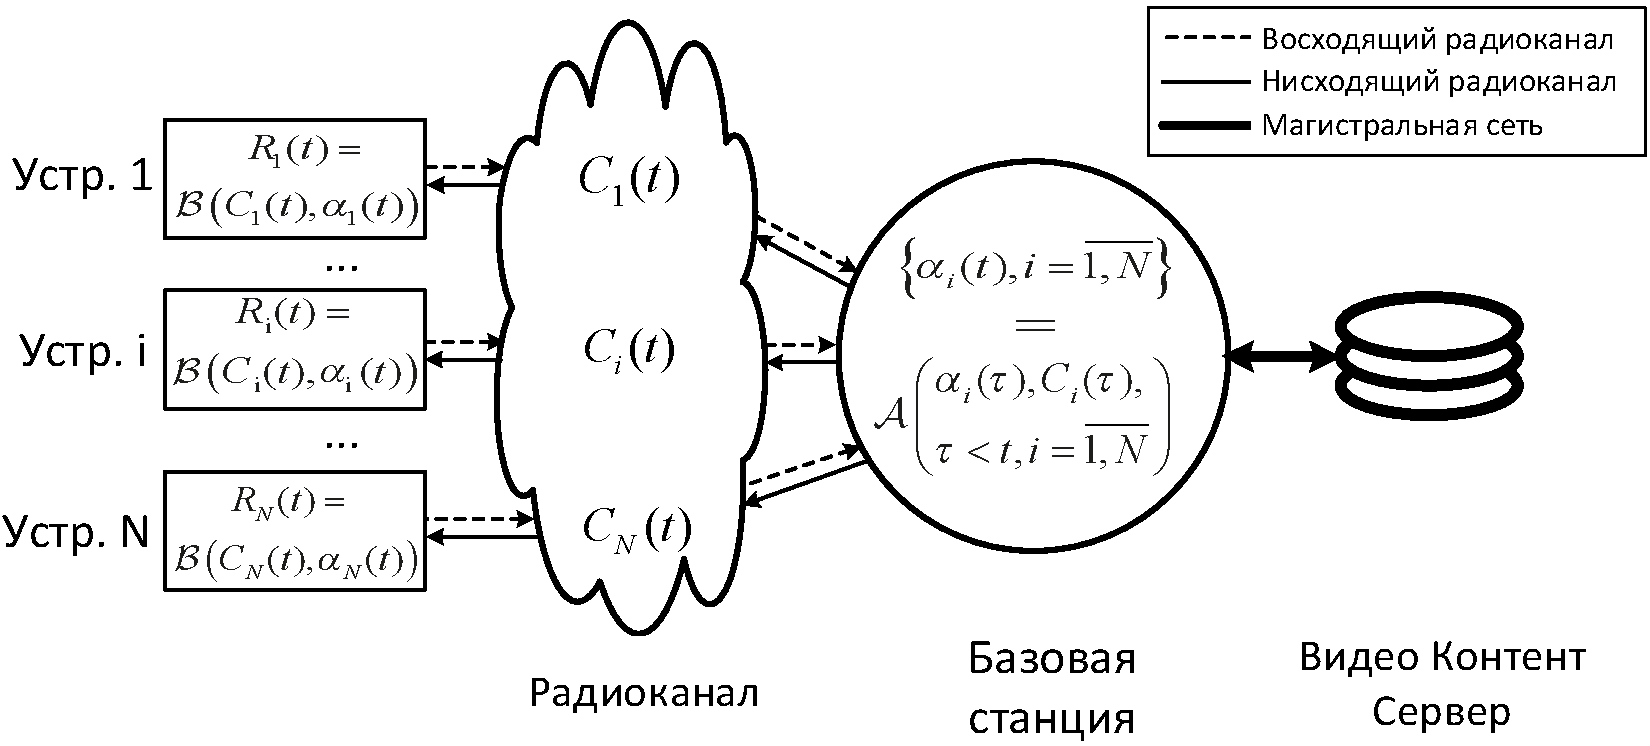
\includegraphics[width=\textwidth]{../Dissertation/images/Chapter2/SystemModelEch.pdf}
\caption{Структура модели передачи видеоданных в централизованных беспроводных сетях}
\label{fig:SystemModel}
\end{center}
\end{figure}

\textbf{Видео контент сервер}. Каждый сегмент видеоданных представлен в непрерывном отрезке битовых скоростей: $R_{i,j} \in [R_{min}, R_{max}], i=\overline{1,N}$.

\textbf{Модель поведения пользователя} характеризуется \textit{коэффициентом разреженности видеопотока пользователя $i$}~--~отношение суммы длительностей просмотра и пауз к длительности просмотра пользователя $i$ за интервал времени $T\rightarrow\infty$:
$$\gamma_i = \lim\limits_{T\rightarrow\infty} \frac{w_i^T + p_i^T}{w_i^T}.$$

Пользователь является активным в момент времени $t$, если он осуществляет загрузку в данный момент, иначе, пользователь считается неактивным.

\textbf{Беспроводная система передачи данных}. В \textit{беспроводном канале} связи затухание сигнала при распространении происходит одинаково по всей ширине полосы передачи данных для конкретного пользователя в одном моменте времени. Введем в рассмотрение величину $C_i(t)$, равную скорости передачи данных по беспроводному каналу, если все доступные ресурсы были выделены $i$-му пользователю в момент времени $t$, которую далее будем называть максимально достижимой скоростью канала.
\newline
Используемые допущения для модели \textit{беспроводного канала}:
\begin{itemize}
	\item При передаче одного пакета $k$ из сегмента $j$ пользователем $i$ в нисходящей линии связи максимально достижимая скорость канала постоянна: $$C_i(t)=C_{i,j,k}, t_{i,j,k} \leq t \leq t_{i,j,k}+\Delta t_{i,j,k},$$
	где $t_{i,j,k}$~--~момент времени начала загрузки пользователем $i$ пакета $k$ из сегмента $j$, $\Delta t_{i,j,k}$~--~длительность загрузки пользователем $i$ пакета $k$ из сегмента $j$, $C_{i,j,k}$~--~максимально достижимая скорость канала пользователя $i$ в течении загрузки пакета $k$ из сегмента $j$.
	\item Последовательности случайных величин: $C^{-1}_{i,1}, C^{-1}_{i,2}, \ldots, i=\overline{1,N},$
	где $C_{i,j}^{-1} = \frac{1}{P_{i,j}}\sum\nolimits_{k=1}^{K_{i,j}} \frac{1}{C_{i,j,k}}$, формируют эргодические случайные процессы с конечными математическими ожиданиями $E[C_i^{-1}]$ и коэффициентами вариации $\nu^{C}_i$ соотвественно.
\end{itemize}

В каждый момент времени $t$, \textit{алгоритм планирования} распределяет доли ресурсов канала $\alpha_i(t)$ для всех пользователей:  $A(t) = \left\{\alpha_{i}(t), i = \overline{1,N}\right\}$. Очевидным ограничением на работу алгоритма планирования является конечность объема доступных ресурсов:
$$\forall t: \sum\nolimits_{i=1}^{N}\alpha_{i}(t) \leq 1.$$
Для решения задачи распределения ресурсов планировщику доступна информация о предыстории, а именно доли выделенных ресурсов канала, значения максимально достижимых скоростей канала и объем переданных данных для каждого пользователя:
\begin{equation}
\nonumber
A(t) = \mathcal{A}\left( \alpha_i(\tau), C_i(\tau);\tau<t, i=\overline{1,N} \right),
\label{eq:SchedulingRule}
\end{equation}
где $\mathcal{A}\left(\cdot\right)$ является алгоритмом планирования.
\newline
Используемые допущения для модели \textit{алгоритма планирования}:
\begin{itemize}
	\item Планировщик распределяет все доступные ресурсы канала в каждый момент времени;
	\item Планировщик не выделяет ресурсы неактивным пользователям;
	\item В любой момент времени каждому активному пользователю гарантируется минимальная доля ресурсов канала.
\end{itemize}

\textbf{Пользовательские устройства}. При заказе видеоплеером нового сегмента видеоданных решается задача выбора битовой скорости для заказываемого сегмента, которая представлена следующим выражением:
\begin{equation}
\nonumber
R_{i,j} = \mathcal{B}\left(R_{i,k}, C_i(\tau), \alpha_i(\tau); k < j, \tau<t_{i,j} \right),
\end{equation}
где $\mathcal{B}\left(\cdot\right)$ является алгоритмом вычисления битовой скорости $j$-го сегмента пользователя $i$, $R_{i,j}$~--~битовая скорость потока $j$-го сегмента пользователя $i$, $t_{i,j}$~--~момент времени заказа пользователем $i$ сегмента под номером $j$.
\newline
Используемые допущения:
\begin{itemize}
	\item Частота переключений битовой скорости ограничена:
	\begin{equation}
	\nonumber
	\forall i: \frac{ \sigma\left[R_{i}\right] }{ E\left[R_{i}\right]} \leq \nu^R_i,
	\label{eq:SwitchRatio}
	\end{equation}
	где $E[R_i] = \lim\nolimits_{j \rightarrow \infty}E[R_{i,j}]$, $\sigma\left[R_{i}\right] = \lim\nolimits_{j \rightarrow \infty}\sigma\left[R_{i,j}\right]$.
	\item Последовательности $R_{i,1}, R_{i,2}, \ldots, i=\overline{1,N}$ формируют эргодические случайные процессы с конечными математическими ожиданиями $E[R_{i}]$ и коэффициентами вариации не превышающими значений $\nu^R_i$ соотвественно.
\end{itemize}

Представленная аналитическая модель описывает важнейшие компоненты и параметры реальной системы передачи видеоданных по протоколу HTTP. Основываясь на данной модели вводится и доказывается утверждение~\ref{lem:GeneralConstrain}.

\begin{lemma}
\label{lem:GeneralConstrain}
Для всевозможных алгоритмов планирования и адаптации видеоряда, удовлетворяющих допущениям, истинно следующее неравенство:
\emph{
\begin{equation}
	\label{eq:GeneralConstrain}
	\nonumber
	\sum\nolimits_{i=1}^{N} {\left(1-\nu^R_i\nu^C_i\right)\frac{E[R_i]E[C_i^{-1}]}{q_i + \gamma_i}} \leq 1.
\end{equation}
}
\end{lemma}

Результат, представленный в утверждении \ref{lem:GeneralConstrain}, описывает взаимосвязь между всеми характеристиками сети передачи видеоданных от особенностей модели поведения пользователя ($\gamma_i$, $q_i$) и характеристик видеопотока ($E[R_i]$), до аспектов работы радиоканала ($E[C_i^{-1}]$) для всех пользователей в сети. Полученное выражение используется в последующих разделах в качестве ограничения на доступный объем ресурсов радиоканала при оптимизации передачи видеоданных в беспроводных централизованных сетях.

\textbf{\textit{Третий раздел}} посвящен исследованию разработке алгоритмов распределения ресурсов радиоканала при передаче неадаптивных видеопотоков для критерия нормированного отношения длительностей буферизации и просмотра \mbox{$g_i$ (выражение \ref{eq:g_def})}.

Рассмотрение передачи неадаптивных видеопотоков приводит к изменению допущения, описывающего выбор битовой скорости для сегментов видеоданных следующим образом: значение битовой скорости видеопотока для каждого конкретного абонента неизменно во времени и равняется: $R_i, i=\overline{1,N}$, следовательно, алгоритм адаптации видеоряда $\mathcal{B}$ является вырожденным и значение $\nu^R_i = 0, i = \overline{1,N}$. В рамках настоящего раздела считается, что коэффициент разреженности видеопотока $\gamma_i$ для всех пользователей имеет равное значение: $\gamma_i = \gamma, i=\overline{1,N}$.

Таким образом, предлагается оценивать производительность алгоритма планирования следующим образом:
$$\bar{g}\left(A\right) = \frac{1}{N}\left(\sum\nolimits_{i=1}^{N} {g_i\left(A\right)}\right),$$
где $A$~--~конкретный алгоритм планирования, установленный на базовой станции.

Задача определения максимально возможной производительности алгоритмов распределения ресурсов радиоканала при передаче неадаптивных видеопотоков сводится к нахождению нижней границы нормированного отношения длительностей буферизации и просмотра:

\begin{equation}
	\label{eq:gMetricGoal}
	G = \inf\limits_{A \in \mathcal{A}} \bar{g}\left(A\right).
\end{equation}

Данная задача может быть представлена в виде оптимизационной задачи нелинейного программирования (\ref{eq:optim_problem_g}), решение которой определяет нижнюю границу нормированного отношения длительностей буферизации и просмотра по множеству алгоритмов $\mathcal{A}$.

\begin{equation}
\begin{array}{l}
\text{ \textbf{Минимизировать:} } G = \frac{1}{N}\sum\nolimits_{i=1}^{N} {g_i} \\
\text{ \textbf{При условии:} }\\
\begin{cases}
\sum\nolimits_{i=1}^{N} {\frac{K_i (1-g_i)}{g_i + \gamma (1-g_i)}} \leq 1 \\
g_i \in [0, 1], i=\overline{1,N}
\end{cases}
\end{array},
\label{eq:optim_problem_g}
\end{equation}
где $K_i = R_i E[C_i^{-1}]$.

Оптимизационная задача (\ref{eq:optim_problem_g}) удовлетворяет критерию жадного выбора и была сведена к обобщенной непрерывной задаче о рюкзаке, в котором целевая функция представлена суммой монотонно возрастающих выпуклых функций. Алгоритм нахождения решения для обобщенной непрерывной задачи о рюкзаке представлен в третье разделе.
%Решение задачи (\ref{eq:optim_problem_g}) может быть найдено на основе <<жадного>> алгоритма. В настоящем разделе задача (\ref{eq:optim_problem_g}) была сведена к решению обобщенной задачи о непрерывном рюкзаке, в котором целевая функция представлена суммой монотонно возрастающих выпуклых функций. Алгоритм нахождения решения для обобщенной задачи о непрерывном рюкзаке представлен в третье разделе. Найденный алгоритм решения обладает низкой вычислительной сложностью, что позволяет на его основе сформировать алгоритм планирования.

Далее предлагается \textbf{алгоритм распределения ресурсов радиоканала}, обладающий большей, чем известные ранее алгоритмы, производительностью для критерия $G$ при передаче неадаптивных видеопотоков. Научная новизна предлагаемого планировщика заключается в использовании концепции \textit{совместного планирования}. Совместное планирование реализуется путем использования решения оптимизационной задачи (\ref{eq:optim_problem_g}) на основе оценок характеристик системы в момент времени $t$ для каждого пользователя $i$: $\hat{R_i}(t)$~--~оценка битовой скорости просматриваемого потока и $\hat{C_i}(t)$~--~оценка максимально достижимой скорости канала. Предлагаемый планировщик представлен алгоритмом \ref{alg:sched}.

\begin{algorithm}
  \caption{: Распределения ресурсов радиоканала в момент времени $t$}
	\label{alg:sched}
  \begin{algorithmic}[1]
	\item Вычисление оценок параметров системы передачи видеоданных для множества активных пользователей $\mathcal{U}(t): \hat{R_i}(t), \hat{C_i}(t), i \in \mathcal{U}(t)$;
	\item Нахождение решения оптимизационной задачи (\ref{eq:optim_problem_g}) для множества пользователей $\mathcal{U}(t):\hat{G}(t) = \{\hat{g}_i(t), i \in \mathcal{U}(t)\}$, при $K_i = \hat{R_i}(t) / \hat{C_i}(t)$ и $\gamma = 1$;
	\item Вычисление долей беспроводного канала:$$\alpha_i(t) = \begin{cases}
					\frac{\hat{R_i}(t) (1 - \hat{g}_i(t)) + S^{min}}{\hat{C_i}(t)}, & i \in \mathcal{U}(t) \\
					0, & i \notin \mathcal{U}(t)
					\end{cases}, i = \overline{1,N},$$
					где $S^{min}$~--~минимально гарантированная скорость получения данных;
	\item Распределение ресурсов радиоканала с учетом значений $\alpha_i(t), i = \overline{1,N}$.
  \end{algorithmic}
\end{algorithm}
Полное описание планировщика приведено в третьем разделе диссертационного исследования. Предложенный алгоритм планирования обладает вычислительной сложностью $O(N \log_{2}N), N \to \infty$ и может быть реализован в режиме реального времени на базовой станции.

Для демонстрации производительности предложенного алгоритма планирования в среде моделирования NS-3, соответствующей стандарту связи LTE, был реализован полный комплекс моделей, введенных во втором разделе, и проведено моделирование типового сценария работы одной соты. В данном сценарии пользователи просматривали последовательность роликов с битовой скоростью 1 Мбит/с, со случайными паузами между ними, абоненты были расставлены на прямой линии по удалению от базовой станции. Была построена зависимость значения критерия качества восприятия $G$ от числа пользователей в соте для разных планировщиков (рисунок \ref{fig:G_PLOT}). Производительность предложенного алгоритма планирования превосходит известные решения на $7-14\%$ по числу удовлетворенных пользователей в соте при зафиксированном значении критерия $G$. Производительность предложенного планировщика близка к найденной нижней границе.
\begin{figure}[htbp]
\begin{center}
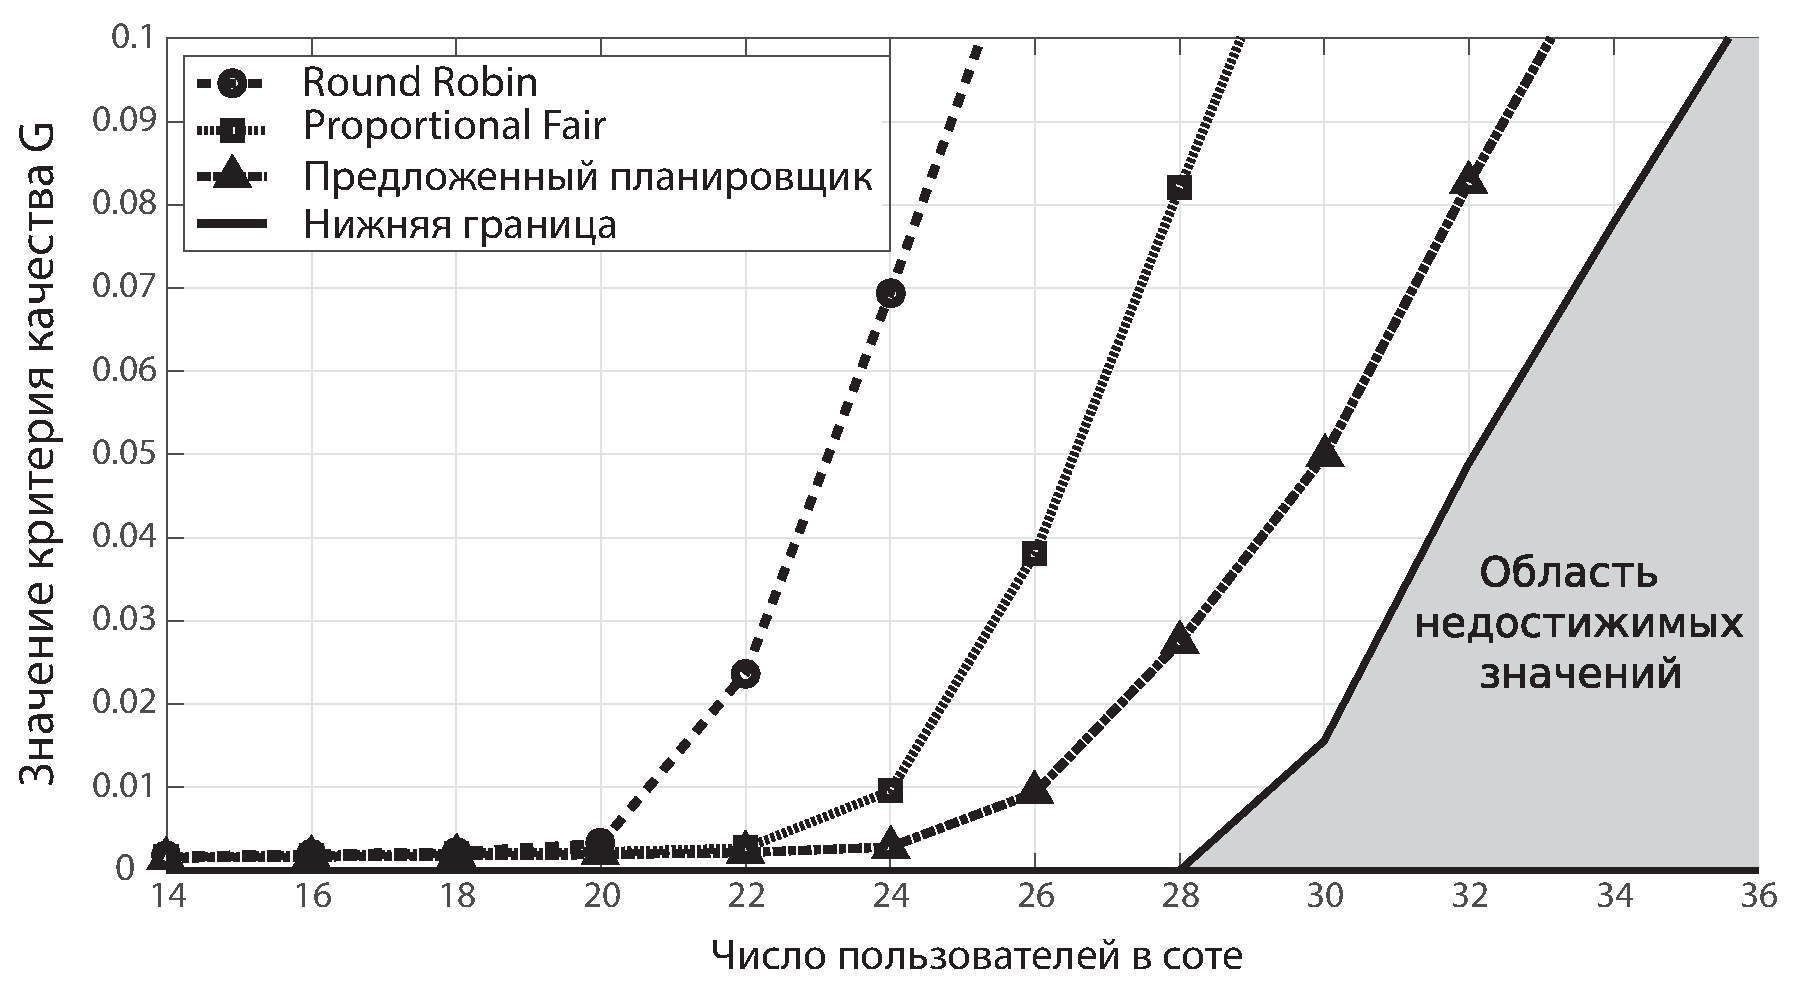
\includegraphics[width=0.7\textwidth]{../Dissertation/images//Chapter3/G_PLOT.pdf}
\caption{Сравнение предложенного алгоритма планирования с известными планировщиками и найденной нижней границей}
\label{fig:G_PLOT}
\end{center}
\end{figure}

\textbf{\textit{Четвертый раздел}} посвящен исследованию алгоритмов распределения ресурсов радиоканала при передаче адаптивных видеопотоков для критерия качества отношение длительностей буферизации и просмотра $q_i$ (выражение \ref{eq:q_def}), с учетом средней битовой скорости просматриваемого потока.

Важно отметить, что ввиду наличия адаптации видеопотока к условиям работы беспроводного канала
%связи возникает обратная связь между работой алгоритма планирования и алгоритма адаптации видеоряда на всех пользовательских устройствах: исходя из скорости передачи информации в беспроводном канале каждый конкретный видеоплеер выбирает битовую скорость запрашиваемого потока, что имеет непосредственное влияние на нагрузку беспроводного канала связи и, как следствие, на скорости передачи данных всех пользователей в соте. Таким образом,
на фактор буферизации оказывают влияние алгоритмы планирования распределения ресурсов $A$ и адаптации видеоряда $B$, принадлежащие множествам $\mathcal{A}$ и $\mathcal{B}$ соответственно.

В соответствии с проведенным исследованием критериев качества восприятия в первом разделе предлагается оценивать производительности системы по двум критериям:
\begin{itemize}
	\item Среднее значение отношения длительности буферизаций к длительности просмотра:
	$$\overline{q}\left(A,B\right) = \frac{1}{N}\left(\sum\nolimits_{i=1}^{N} {q_i\left(A, B\right)}\right).$$
	\item Среднее значение битовой скорости просматриваемого видеопотока:
	$$\overline{R}\left(A,B\right) = \frac{1}{N}\left(\sum\nolimits_{i=1}^{N} {E\left[R_i\left(A, B\right)\right]}\right).$$
\end{itemize}

Основная задача настоящего раздела заключается в нахождении нижней границы по всевозможным алгоритмам планирования и адаптации видеоряда, удовлетворяющим допущениям введенным во втором разделе, среднего отношения длительностей буферизации и просмотра по всему множеству абонентов в системе, при условии, что средняя битовая скорость просматриваемого потока по всем пользователям не меньше заданного значения $R_{avg}$ (\ref{eq:extr_param}).
\begin{equation}
Q = \inf\limits_{A,B: \overline{R}\left(A,B\right) \geq R_{avg}, A \in \mathcal{A}, B \in \mathcal{B}} \overline{q}\left(A,B\right).
\label{eq:extr_param}
\end{equation}

Задача нахождения нижней границы критерия качества восприятия $Q$ может быть представлена в виде оптимизационной задачи (\ref{eq:optim_problem_q}).

\begin{equation}
\begin{array}{l}
\text{ \textbf{Минимизировать:} } Q = \frac{1}{N}\sum\nolimits_{i=1}^N q_i \\
\text{ \textbf{При условии:} }\\
\begin{cases}
\sum\nolimits_{i=1}^{N} {\left(1-\nu^R_i\nu^C_i\right)\frac{\tilde{R}_i \tilde{C}^{-1}_i }{q_i + \gamma_i}} -1 \leq 0 \\
-\frac{1}{N}\sum\nolimits_{i=1}^{N}\tilde{R}_i + R_{avg} \leq 0 \\
\tilde{R}_i \in \left[R_{min}, R_{max}\right], i=\overline{1,N} \\
-q_i \leq 0,\mbox{ }i=\overline{1,N} \\
\end{cases}
\end{array},
\label{eq:optim_problem_q}
\end{equation}
где $\tilde{R}_i = E[R_i]$ и $\tilde{C}^{-1}_i = E[C^{-1}_i]$.

Нелинейная оптимизационная задача (\ref{eq:optim_problem_q}) относится к классу невыпуклых задач с ограничениями общего вида. К сожалению, для данного класса задач не существует стандартных методов решения, поэтому в настоящем разделе было предложено решение задачи (\ref{eq:optim_problem_q}), основанное на двухступенчатой оптимизации:
\begin{itemize}
	\item Введение промежуточной оптимизационной задачи, которая имеет известный алгоритм решения;
	\item Нахождение взаимосвязи между решениями оптимизационной задачи и промежуточной;
	\item Постановка оптимизационной задачи с ослабленными ограничениями и нахождение ее решения.
\end{itemize}
В заключении четвертого раздела предлагается алгоритм решения оптимизационной задачи (\ref{eq:optim_problem_q}) и производится сравнение производительности существующих эвристик распределения ресурсов беспроводного канала по критерию $Q$ с найденной границей для адаптивных видеопотоков с известной нижней границей и существующими эвристиками для неадаптивного видео (рисунок \ref{fig:Q_PLOT}). В сценарии, описанном в третьем разделе, было зафиксировано число пользователей в соте и произведено моделирование эвристических алгоритмов планирования при передаче адаптивного видео. Моделирование эвристик при передаче неадаптивного видео было выполнено в предположении, что битовая скорость видеопотоков, просматриваемых всеми пользователями, равняется $R_{avg}$.

%В аналогичных условиях было произведено моделирование для эвристик при передаче неадаптивного видео, когда просматриваемая битовая скорость потоков всех пользователей равнялась значению $R_{avg}$.
\begin{figure}[H]
\begin{center}
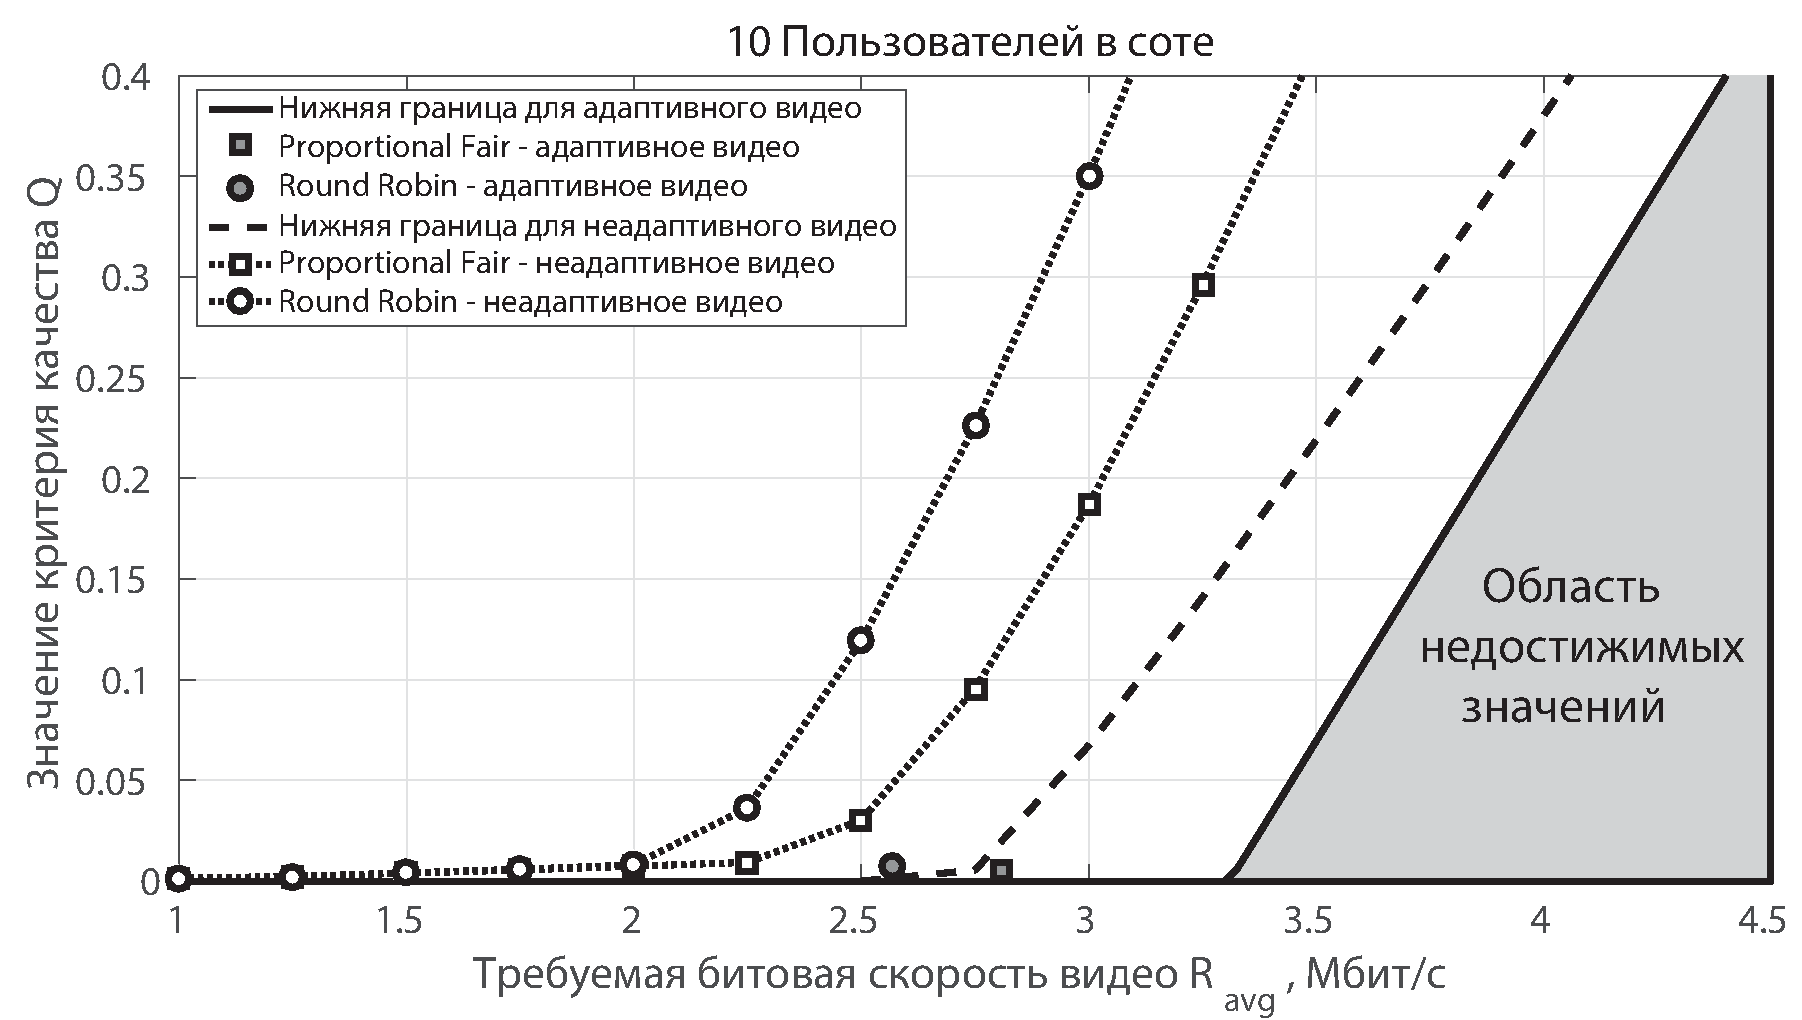
\includegraphics[width=0.7\textwidth]{../Dissertation/images/Chapter4/10_Users_v2.pdf}
\caption{Сравнение производительности известных алгоритмов планирования при передаче адаптивного видео с нижней границей}
\label{fig:Q_PLOT}
\end{center}
\end{figure}
Использование адаптивной технологии передачи видео позволяет достичь большей производительности алгоритмов планирования и, как следствие, сети передачи данных в целом. Планировщик \textit{Proportional Fair} обладает большей производительностью в сравнении с алгоритмом \textit{Round Robin}, и демонстрирует производительность близкую к нижней границе критерия качества $Q$ (рисунок \ref{fig:Q_PLOT}).

В \textbf{\textit{заключении}} приведены основные результаты, полученные в диссертационной работе.
%------------------------------------------------------------------------------------------------------------------------------------%
%\newpage
%\begin{center}
%    \large\bf ОСНОВНЫЕ РЕЗУЛЬТАТЫ РАБОТЫ
%\end{center}
\subsection*{Основные результаты работы}

%\smallskip

%Основные результаты, полученные в диссертационной работе, можно сформулировать следующим образом.
%% Согласно ГОСТ Р 7.0.11-2011:
%% 5.3.3 В заключении диссертации излагают итоги выполненного исследования, рекомендации, перспективы дальнейшей разработки темы.
%% 9.2.3 В заключении автореферата диссертации излагают итоги данного исследования, рекомендации и перспективы дальнейшей разработки темы.
\begin{enumerate}
    \item Предложена модель беспроводной централизованной сети связи при передаче видеоданных по протоколу HTTP. Найдена взаимосвязь между объективными характеристиками сети и качеством воспроизведения видео. Предложенная модель и найденная взаимосвязь позволяют производить аналитические исследования производительности беспроводных централизованных сетей при доминировании передачи видеоданных.
    \item Предложены алгоритмы вычисления граничных значений максимально возможной производительности беспроводных централизованных сетей для следующих критериев качества восприятия:
    \begin{itemize}
	    \item Нормированное отношение длительности буферизации к просмотру при передаче неадаптивных видеопоследовательностей;
	    \item Отношение длительности буферизации к просмотру с учетом средней битовой скорости видео при передаче адаптивного видео.
    \end{itemize}
    Полученные результаты могут быть использованы в качестве опорных значений при разработке новых алгоритмов планирования, учитывающие тип передаваемого трафика и требования к его обслуживанию, для существующих и последующих стандартов беспроводной связи.
    \item Предложен алгоритм планирования распределения ресурсов беспроводного канала, позволяющий минимизировать нормированное отношение длительности буферизации к просмотру при передаче неадаптивного видео. Предложенный алгоритм позволяет увеличить емкость соты на $7-14\%$ в сравнении с известными решениями и демонстрирует производительность близкую к найденной аналитической границе.
\end{enumerate}


\renewcommand*{\refname}{\vspace*{-13mm}}

%\newpage
\renewcommand{\refname}{\large Публикации автора по теме диссертации}
Основное содержание работы изложено в следующих \textbf{публикациях} (статьи 1-2 опубликованы в изданиях, включенных в перечень ВАК, работы 3-5 индексируются в Scopus):
\nocite{*}
\insertbiblioauthor                          % Подключаем Bib-базы
%\insertbibliofull
